%%%%%%%%%%%%%%%%%%%%%%%%%%%%%%%%%%%
%This is the LaTeX ARTICLE template for RSC journals
%Copyright The Royal Society of Chemistry 2016
%%%%%%%%%%%%%%%%%%%%%%%%%%%%%%%%%%%

\documentclass[twoside,twocolumn,9pt]{article}
\usepackage{tgheros}
\usepackage[utf8]{inputenc}
\renewcommand{\familydefault}{\sfdefault}

\usepackage{extsizes}
\usepackage[super,sort&compress,comma]{natbib} 
\usepackage[version=3]{mhchem}
\usepackage[left=1.5cm, right=1.5cm, top=1.785cm, bottom=2.0cm]{geometry}
\usepackage{balance}
\usepackage{mathptmx}
\usepackage{sectsty}
\usepackage{graphicx} 
\usepackage{lastpage}
\usepackage[format=plain,justification=justified,singlelinecheck=false,font={stretch=1.125,small,sf},labelfont=bf,labelsep=space]{caption}
\usepackage{float}
\usepackage{fancyhdr}
\usepackage{fnpos}
\usepackage[english, german]{babel}
\addto{\captionsenglish}{%
  \renewcommand{\refname}{Notes and references}
}
\usepackage{array}
\usepackage{droidsans}
\usepackage{charter}
\usepackage[T1]{fontenc}
\usepackage[usenames,dvipsnames]{xcolor}
\usepackage{setspace}
\usepackage[compact]{titlesec}
%%%Please don't disable any packages in the preamble, as this may cause the template to display incorrectly.%%%


\usepackage{xcolor}
\definecolor{ugent_blue}{RGB}{30, 100, 200}
\definecolor{ugent_yellow}{cmyk}{.0, .10, 1, 0}

\usepackage{titlesec}
\titleformat{\section}
{\color{ugent_blue}\normalfont\Large\bfseries}
{\color{ugent_blue}\thesection}{1em}{}

\usepackage[colorlinks=true,linkcolor=black,citecolor=ugent_blue]{hyperref}

%\AtEveryCite{\color{ugent_blue}}




\usepackage{epstopdf}%This line makes .eps figures into .pdf - please comment out if not required.

\definecolor{cream}{RGB}{222,217,201}

\begin{document}

\pagestyle{fancy}
\thispagestyle{plain}
\fancypagestyle{plain}{
%%%HEADER%%%
\renewcommand{\headrulewidth}{0pt}
}
%%%END OF HEADER%%%

%%%PAGE SETUP - Please do not change any commands within this section%%%
\makeFNbottom
\makeatletter
\renewcommand\LARGE{\@setfontsize\LARGE{15pt}{17}}
\renewcommand\Large{\@setfontsize\Large{12pt}{14}}
\renewcommand\large{\@setfontsize\large{10pt}{12}}
\renewcommand\footnotesize{\@setfontsize\footnotesize{7pt}{10}}
\makeatother

\renewcommand{\thefootnote}{\fnsymbol{footnote}}
\renewcommand\footnoterule{\vspace*{1pt}% 
\color{cream}\hrule width 3.5in height 0.4pt \color{black}\vspace*{5pt}} 
\setcounter{secnumdepth}{5}

\makeatletter 
\renewcommand\@biblabel[1]{#1}            
\renewcommand\@makefntext[1]% 
{\noindent\makebox[0pt][r]{\@thefnmark\,}#1}
\makeatother 
\renewcommand{\figurename}{\small{Fig.}~}
\sectionfont{\sffamily\Large}
\subsectionfont{\normalsize}
\subsubsectionfont{\bf}
\setstretch{1.125} %In particular, please do not alter this line.
\setlength{\skip\footins}{0.8cm}
\setlength{\footnotesep}{0.25cm}
\setlength{\jot}{10pt}
\titlespacing*{\section}{0pt}{4pt}{4pt}
\titlespacing*{\subsection}{0pt}{15pt}{1pt}
%%%END OF PAGE SETUP%%%

%%%FOOTER%%%
\fancyfoot{}
\fancyfoot[LO,RE]{\vspace{-7.1pt}
\includegraphics[height=9pt]{head_foot/LF}}
\fancyfoot[CO]{\vspace{-7.1pt}\hspace{11.9cm}
\includegraphics{head_foot/RF}}
\fancyfoot[CE]{\vspace{-7.2pt}\hspace{-13.2cm}
\includegraphics{head_foot/RF}}
\fancyfoot[RO]{\footnotesize{\sffamily{1--\pageref{LastPage} {\color{ugent_yellow} ~\textbar } \hspace{2pt}\thepage}}}
\fancyfoot[LE]{\footnotesize{\sffamily{\thepage~{\color{ugent_yellow} ~\textbar }\hspace{4.65cm} 1--\pageref{LastPage}}}}
\fancyhead{}
\renewcommand{\headrulewidth}{0pt} 
\renewcommand{\footrulewidth}{0pt}
\setlength{\arrayrulewidth}{1pt}
\setlength{\columnsep}{6.5mm}
\setlength\bibsep{1pt}
%%%END OF FOOTER%%%

%%%FIGURE SETUP - please do not change any commands within this section%%%
\makeatletter 
\newlength{\figrulesep} 
\setlength{\figrulesep}{0.5\textfloatsep} 

\newcommand{\topfigrule}{\vspace*{-1pt}% 
\noindent{\color{cream}\rule[-\figrulesep]{\columnwidth}{1.5pt}} }

\newcommand{\botfigrule}{\vspace*{-2pt}% 
\noindent{\color{cream}\rule[\figrulesep]{\columnwidth}{1.5pt}} }

\newcommand{\dblfigrule}{\vspace*{-1pt}% 
\noindent{\color{cream}\rule[-\figrulesep]{\textwidth}{1.5pt}} }

\makeatother
%%%END OF FIGURE SETUP%%%

%%%TITLE, AUTHORS AND ABSTRACT%%%
\twocolumn[
  \begin{@twocolumnfalse}
{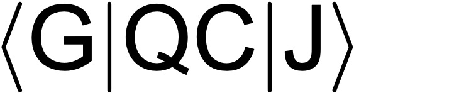
\includegraphics[height=30pt]{head_foot/journal_name}\hfill\raisebox{0pt}[0pt][0pt]{
\includegraphics[height=55pt]{head_foot/RSC_LOGO_CMYK}}\\[1ex]

\includegraphics[width=18.5cm]{head_foot/header_bar}}\par
\vspace{1em}
\sffamily
\begin{tabular}{m{4.5cm} p{13.5cm} }

& \noindent\LARGE{\textbf{This is the title$^\dag$}} \\%Article title goes here instead of the text "This is the title"
\vspace{0.3cm} & \vspace{0.3cm} \\

& \noindent\large{Full Name,$^{\ast}$\textit{$^{a}$} Full Name,\textit{$^{b\ddag}$} and Full Name\textit{$^{a}$}} \\%Author names go here instead of "Full name", etc.

& \\

& \noindent\normalsize{Do \emph{not} write an abstract. That will be done when the outline has matured into a completed paper.} \\%The abstrast goes here instead of the text "The abstract should be..."

\end{tabular}

\end{@twocolumnfalse} \vspace{1.6cm}

  ]
%%%END OF TITLE, AUTHORS AND ABSTRACT%%%

%%%FONT SETUP - please do not change any commands within this section
\renewcommand*\rmdefault{bch}\normalfont\upshape
\rmfamily
\section*{}
\vspace{-1cm}


% %%%FOOTNOTES%%%

\footnotetext{\textit{$^{a}$~Ghent Quantum Chemistry Group, Krijgslaan 281 (S3), B-9000 Gent, België}}
\footnotetext{\textit{$^{b}$~Corresponding author:} \texttt{firstname.lastname@ugent.be}}

% %Please use \dag to cite the ESI in the main text of the article.
% %If you article does not have ESI please remove the the \dag symbol from the title and the footnotetext below.
% \footnotetext{\dag~Electronic Supplementary Information (ESI) available: [details of any supplementary information available should be included here]. See DOI: 00.0000/00000000.}
% %additional addresses can be cited as above using the lower-case letters, c, d, e... If all authors are from the same address, no letter is required

% \footnotetext{\ddag~Additional footnotes to the title and authors can be included \textit{e.g.}\ `Present address:' or `These authors contributed equally to this work' as above using the symbols: \ddag, \textsection, and \P. Please place the appropriate symbol next to the author's name and include a \texttt{\textbackslash footnotetext} entry in the the correct place in the list.}


%%%END OF FOOTNOTES%%%

%%%MAIN TEXT%%%%


\section{Introduction}

\paragraph*{}
When thinking about chemistry, one always thinks in terms of atoms, that are bonded together in molecules. In order to correctly predict the behaviour of 
thes entities we will need to know what they look like. How are the atoms aranged in a molecule? Why are they arranged in this way? The answer to these
questions lies in the Shrödinger equation, \eqref{eq:erwin}.
\begin{equation}\label{eq:erwin}
  \hat{H}\Psi = E\Psi
\end{equation} 
The Shrödinger equation allows us to express the energy of a wave function. However, it is not exactly solvable for systems that contain one or more electrons,
i.e. all relevant systems. The reason for this is the repulsion that exists between two electrons. This term makes it impossible to solve the Shrödinger equation
analytically for most systems. That is why we need to make approximations. In this paper we will make use of the Hartree-Fock method, which accounts for this
interaction by means of a coulomb operator, \eqref{eq:coulomb}, which accounts for the electronic repulsion between electrons and an exchange operator,
\eqref{eq:exchange}, which accounts for stabilisation between electrons with the same spin. 
\begin{equation}\label{eq:coulomb}
  \hat{J}_j\psi_i(1) = \int\psi_j(2)^*\boldsymbol{r}_{12}^{-1}\psi_j(2)d2 \psi_i(1)
\end{equation}
\begin{equation}\label{eq:exchange}
  \hat{K}_j\psi_i(1) = \int\psi_j(2)^*\boldsymbol{r}_{12}^{-1}\psi_i(12d2 \psi_j(1)
\end{equation}
We can define an expectation value over the Hamiltonian and state that if we are in an energy minimum a small variation in the wave function will not induce a change
in energy \eqref{eq:hamexp}.
\begin{equation}\label{eq:hamexp}
  \langle\psi + \delta\psi|\hat{H}|\psi + \delta\psi \rangle = E + \delta E + \delta E^* + \delta E^2
\end{equation}
In first order we say that if $\psi$ is an eigenfunction of $\hat{H}$, $\delta E$ will equal zero. We will not go into any further detail here.
This approximation might take us a long way in the right direction, but does it take us all the way there? Here we need to introduce different methods within the
Hartree-Fock theory. Restricted Closed shell Hartree-Fock (RHF) forces the electrons into the same orbitals, thus creating doubly occupied orbitals. Even though this 
picture is a chemically logical one, since in chemistry we think about electrons in pairs, physically there is no obligation for the electrons to exist in these pairs.
When we let go of the restriction, we enter the Unrestricted Hartree-Fock method (UHF). This  is no longer confined to closed shell species since it has no problem with 
electrons that do not exist in pairs. However, we see that the wave function in this method does not contain the right symmetries. It paints a physical picture, yet the
chemical intuition is tossed out of the window. This phenomenon is called spin-contamination.
\paragraph*{}
In this particular paper we will take a look at the symmetry in the Hamiltonian. We know that in molecules there can be a lot of symmetry. This symmetry also exists in that 
molecules Hamiltonian, and thus also in every eigenfunction. Now we can easily state that every approximation we make of these eigenfunctions must contain that same symmetry. 
If we aspire to create somthing that is close to reality, but end up with something that does not have any real symmetry, we can do better. The important relation here is that 
the Hamiltonian commutes with the $\hat{S}^2$ operator, meaning that these operators share a complete set of eigenfunctions. Thus an eigenfunction of the Hamiltonian must also
be an eigenfunction of $\hat{S}^2$. We can express this using a commutator \eqref{eq:commut}.
\begin{equation}\label{eq:commut}
  [\hat{H}, \hat{R}] = 0
\end{equation}
We pick the operator $\hat{R}$ as being a certain symmetry operator. Looking back at equation \eqref{eq:hamexp} and the constraint we applied, namely that $\delta E$ should 
remain zero, one can wonder whether equation \eqref{eq:commut} also still holds. Is the slightly varied wave function still an eigenfunction of the symmetry operator as well.
This leads us to Löwdins symmetry dilemma \cite{Lowdin1963}. When we enforce the symmetry and the energy constraint at the same time, the minimum energy we reach is not the
global minimum. However when we drop the symmetry constraint and only enforce the energy, we will reach a lower energy, but will lose all the information with regard to the
symmetry of the system.

\paragraph*{}
We need some kind of theory to bring the best of both worlds together. One one side, we have the chemical intution in the restricted wave functions, on the other the physical
truth in the unrestricted wave functions. Roothaans Restricted Opens Shell theory (ROHF)\cite{Roothaan1960} was an early attempt. However, more recently Tsuchimochi and Scuseria
presented their Constrained Unrestricted Hartree Fock theory (CUHF)\cite{Scuseria2010}. A lot has been said already about this method\cite{Plakhutin2014, Scuseria2011}. In CUHF we
se the spin-contamination to zero. In this work we will use the CUHF wave function as a reference for Single excitation Configuration Interaction (CIS). We will generate the single
excitation energies for the CUHF wave function and compare them to the ROHF and UHF excitations of the same system. 

\paragraph*{}
In this paper we will begin by explaining the theory needed to understand the aformentioned concepts. We will then demonstrate the impact of spin-contamination using the hydrogen gas
dicossiation problem in the different Hartree-Fock modes. After that we will compare the CIS results for UHF, CUHF and ROHF. From there we will be able to verify whether it makes
sense to use CUHF as a reference next to ROHF and UHF. 


\section{Theory}

\subsection{Spin-Contamination}
In general one can define the expectation value of $\hat{S}^2$ like equation \eqref{eq:spinexp}\cite{Andrews1991}.
\begin{equation}\label{eq:spinexp}
    \langle S^2 \rangle = S_z^2 + S_z + q - \sum_{ij}^{pq} S_{ij}^2
\end{equation}
This equation holds for all systems with $q$ beta electrons and $p$ alpha electrons. When the overlap is diagonal, the last terms vanish and we are left with $S_z(S_z + 1)$. 
Spin-contamination is then defined as Equation \eqref{eq:spincont}.
\begin{equation}\label{eq:spincont}
    \delta_s = \langle S^2 \rangle - S_z(S_z + 1)
\end{equation}
As a consequence, UHF suffers a lot from spin contamination. When the alpha and beta orbitals are not the same, the overlap matrix $S$ will not be diagonal. One can not expect the 
last two terms in equation \eqref{eq:spinexp} to vanish, which will result in $\delta_s$ not being equal to zero. This also means that the wave function is no longer an eigenfunction 
of $\hat{S^2}$, as we have seen before. We lose a quantum number and with it the symmetry of the system. We can rewrite spin-contamination as Equation \eqref{eq:spincont2}\cite{Savin2010}.
\begin{equation}\label{eq:spincont2}
    \delta_s = N_\beta - Tr(\gamma^\alpha\gamma^\beta)
\end{equation}
In this equation, $\gamma^{\alpha}$ and $\gamma^\beta$ are the one particle density matrices. In the NO basis, these matrices are block diagonal \cite{Scuseria2010}, with blocks that
can be seen in equations \eqref{eq:gammaa} and \eqref{eq:gammab}, where i corresponds to a certain closed shell orbital. The $gamma^\alpha$ also contains a block that is a 
unity matrix with dimensions $n\times n$ where n is the amount of singly occupied orbitals. In $\gamma^\beta$ this block is a zero matrix of the same dimensions.
\begin{subequations}
  \begin{align}
  \label{eq:gammaa}
  \gamma^\alpha_i &= \begin{bmatrix}
    n_i & m_i \\
    m_i & 1- n_i
  \end{bmatrix}&& \\
  \label{eq:gammab}
  \gamma^\beta_i &= \begin{bmatrix}
    n_i & -m_i \\
    -m_i & 1-n_i
  \end{bmatrix}&&
\end{align}
\end{subequations}
 In these equations $n_i$ is the occupation of orbital i and $m_i = \sqrt{n_i - n_i^2}$\cite{Scuseria2010} We can the define the spin density matrix $M = (\gamma^\alpha - \gamma^\beta)/2$. It is obvious then that equation \eqref{eq:mmatrix} then holds.
 \begin{equation}\label{eq:mmatrix}
   M_i = \begin{bmatrix}
     0 & m_i \\
     m_i & 0
   \end{bmatrix}
 \end{equation}
Using this information we can rewrite equation \eqref{eq:spincont2} to equation \eqref{eq:spincont3}\cite{Scuseria2010}.
\begin{equation}\label{eq:spincont3}
  \delta_s = N_\beta - (N_\alpha + N_\beta)/2 + 2*Tr(M^2)
\end{equation}
In an additional step, we can use algebra to find equation \eqref{eq:spincontfinal}.
\begin{equation}
  \delta_s = 4\sum^{N_{cp}}_i m_i^2
\end{equation}
Now if we want to make the spin contamination zero, we have to eneforce double occupation or no occupation at all. The $N_{cp}$ are the closed shell orbitals. We see here that in 
the closed shell itself, we can no longer have a difference between alpha and beta orbitals. This will be the constraint that gives us the CUHF method.

\subsection{Constrained Unrestricted Hartree Fock}
When talking about CUHF, there is more then one way to make sure that the spin-contamination remains zero. Scuseria and Tsuchimochi will enforce the constraint we mentioned in the 
last section, where they allow only doubly occupied orbitals in the closed shell\cite{Scuseria2010}. It can be shown that the normal UHF energy can be constructed by adding a 
correlation energy term to the closed shell energy. These terms can be seen in equations \eqref{eq:cseng} and \eqref{eq:correng}\cite{Savin2010}.
\begin{subequations}
  \begin{align}
    \label{eq:cseng}
    E_{cs} &= 2\sum_{ij}h_{ij}P_{ij} + \sum_{ijkl}(2\langle ij|kl\rangle - \langle ij|lk \rangle)P_{ik}P_{jl}&&\\
    \label{eq:correng}
    E_c &= -\sum_{ijkl}\langle ij|lk \rangle M_{ik}M_{jl}&&
  \end{align}
\end{subequations}
Where the matrix $M$ is the spin density matrix (cfr. supra) and the $P$ matrix is the charge density matrix: $P = (\gamma^\alpha + \gamma^\beta)/2$. 

\section{Methodology}

How were methods/descriptors implemented and characterized? Which systems are of interest for this hypothesis?
\paragraph*{}
The $H_3$ radical will be used as a model system. This is a small molecule that allows for easy interpretation and oversight. We will also use a limited basis, sto-3g, for these same reasons.
\section{Results and discussion}

Central ideas: What were the results? Organize the outline and the paper around easily assimilated data - tables, equations, figures, schemes - rather than around text. Organize in order of importance, not in chronological order.

\begin{itemize}
    \item The $H_2$ stretch in different HF modes.
    \item The excited states in different HF modes
    \item Spin contamination in the excited states
\end{itemize}

\subsection{$H_2$ Stretch}
We will demonstrate the effect of spin contamination using the stretch of the dihydrogen molecule.
\begin{center}
  \begin{figure}[h]
      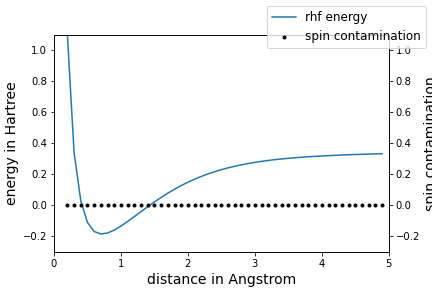
\includegraphics[width=\linewidth]{./../notes/figures/rhf.png}
      \caption{The RHF energy against the distance in an $H_2$ stretch. The zero level was chosen as the energy of two separate hydrogen atoms.}
      \label{fig:rhfstretch}
  \end{figure}
\end{center}
In Figure \ref{fig:rhfstretch} we can see that the RHF solution is not physically valid. Indeed, we expect the energy to evolve towards the energy of two seperate hydrogen atoms, which clearly does not happen. However we see that the spin contamination is zero, so the wave function has the correct symmetry. The reason for this is simple. We artificially trap the electrons in the same orbital.
\begin{center}
\begin{figure}[h]
  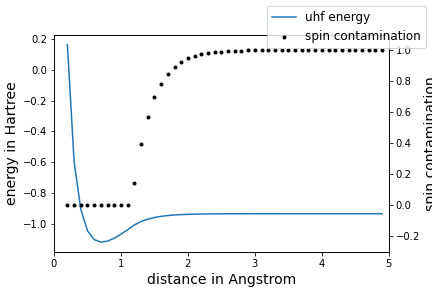
\includegraphics[width=\linewidth]{./../notes/figures/uhf.png}
  \caption{The UHF energy against the distance in an $H_2$ stretch}
  \label{fig:uhfstretch}
\end{figure}
\end{center}
Figure \ref{fig:uhfstretch} shows a physically more correct result. We see that the system does evolve towards two hydrogen atoms. Howver, the spin contamination is rising, and after a certain point reaches the value one. This means that the wave function does no longer have the right symmetry, ergo it is no longer the right wave function.
\begin{center}
\begin{figure}[h]
  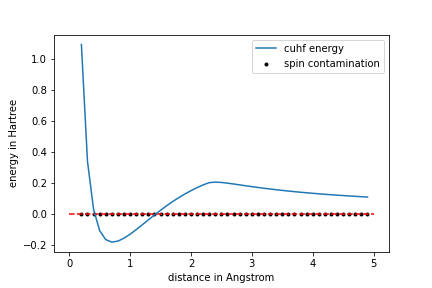
\includegraphics[width=\linewidth]{./../notes/figures/cuhf_mix.png}
  \caption{The CUHF energy against the distance in an $H_2$ stretch}
  \label{fig:cuhfstretch}
\end{figure}
\end{center}
The CUHF picture in Figure \ref{fig:cuhfstretch} is difficult to interpret. We see that the spin contamination remains zero. The energy seems to follow the RHF pattern (see also Figure \ref{fig:combo}) untill a certain point. Then it starts to exponantially decline. Physically this seems like a logical behaviour, as it is now again eveolving to two separate hydrogen atoms. 
\begin{center}
\begin{figure}[h]
  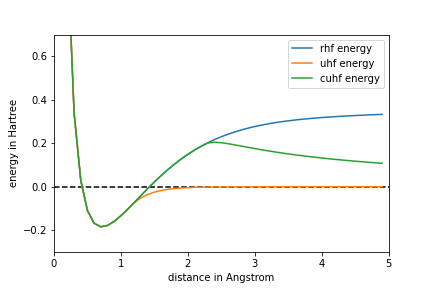
\includegraphics[width=\linewidth]{./../notes/figures/combo.png}
  \caption{The stretch energies plotted together}
  \label{fig:combo}
\end{figure}
\end{center}
For comparison we plotted all the stretches in one plot, Figure \ref{fig:combo}. Here we can see that they all describe short bond lengths correctly, but as the internuclear distance increases, there are deviations visible.
\subsection{CIS results}
We need to plot the excitation energies of $H_3$, together with the ground state energy. This will be done for UHF, CUHF and ROHF, as soon as we can verify our data.
\begin{itemize}
    \item Method implementation
    \paragraph*{}
    For the code we used python with the help of the psi4 package.
    \item Method characterization
    \item System characterization
    \item Results
\end{itemize}
\paragraph*{Figures}
\begin{itemize}
    \item Excitation energies in all modes 
    \item orbitals?
\end{itemize}
\paragraph*{Schemes}
\begin{itemize}
  \item electron configurations for different modes (learn to draw them!!)
\end{itemize}



\section{Conclusions}

Central ideas: What does it all mean? What hypotheses were proved or disproved? What did I learn? Why does it make a difference?


%%%END OF MAIN TEXT%%%

%The \balance command can be used to balance the columns on the final page if desired. It should be placed anywhere within the first column of the last page.

\balance

%If notes are included in your references you can change the title from 'References' to 'Notes and references' using the following command:
%\renewcommand\refname{Notes and references}

%%%REFERENCES%%%
\bibliography{outline} %You need to replace "rsc" on this line with the name of your .bib file
\bibliographystyle{aip} %the AIP's .bst file

\end{document}
